\chapter{结论与展望}\label{chap:future}
%icache目前还是直接映射的。
%被诟病的微结构
%截至中期,工程实现依旧采用的是直接映射的存储结构,后期会将其调整为4路组相连结构。这里有两个目的。其一,risc-v对于页表的规定固定为4KB,为了做到cpu的tlb虚实转化和访问cache的并行,所以cache core的每一路的容量都至多是4KB,也就是说用虚实地址共享的地址(不用tlb cam来进行虚实转换)来索引cache core。但是4KB的容量显然不够的,但是每一路至多4KB,当然可以用硬件来解决顶着色对每一路的cache core进行扩容,但是这就很复杂了。所以另一种思路就是增加路数,比如四路;其二,四路比一路cache的替换率要低,这不光是容量的问题,四路的每路4KB的cache在一般情况下要比容量相同的16KB的单路cache的替换率都低。

%所以对于cache core最终的组织形式目前的想法是4路组相连,每一路4KB,采用LRU或者随机替换或者一种兼而有之的方法。不会参考alpha21464一样做路预测,一是为了降低复杂度,二是因为估计在自己的设计中延迟时序允许。
%基于CAM的重命名表
%更侧重微结构的设计

通过第\ref{chap:analysis}章的分析,相比于单发射五级静态流水线再到双发射五级静态流水线,双发射乱序处理器后端对前端的阻塞大大降低了,但是目前分支预测正确率不高的几个程序运行效率都没有达到预期的提升。

目前已经有很多具体的工作正在实施或者筹划中,但是很遗憾地来不及展示在本文中,如:
\begin{enumerate}[label=(\arabic*)]
	\item 指令高速缓存真正做到四路组相连的结构,每一路4KB。
	\item 参考文献\citet{Alpha21264,MIPS1996},构建高效的内部内存系统(Inner Memory System).
	\item 处理器对外支持整套AXI接口,同时仿真平台也能够支持整套以AXI总线交互的外设,如带延迟的内存。乱序的引入很大程度上就是为了通过硬件的调度来隐藏访存延迟。一旦访存带有延迟,支持四路组相连的数据高速缓存,BIAN相比于顺序流水的CHIWEN和FUXI效率会高不少。从研究的角度来看,实验结果更漂亮;同时从实际应用的角度来看,也更加具有实用性。
	\item 参考章节\ref{subsec:ISA}中介绍RISC-V的特权部分,使BIAN处理器支持MMU和虚拟内存管理。
	\item 尝试去移植在Rocket和BOOM中的仿真外设,真正做到系统的模拟仿真。
	\item 在设计过程中,被诟病最多的一点是rename级的基于RAM形式的重命名表,加上旁路技术读寄存器堆的设计。这里,已经构思好了两部分的解决方案。第一,将重命名表从RAM形式改为CAM形式,CAM形式在后来的讨论中被证实是时序更好,面积更小的方案。第二,取消在rename阶段的旁路,见框图\ref{fig:bian_over2}。
	\begin{figure}[!htbp]
		\centering
		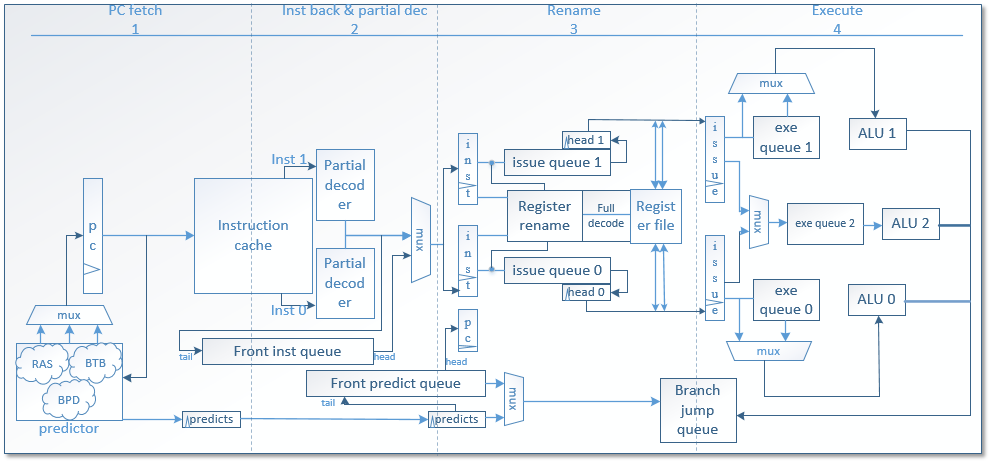
\includegraphics[width=\linewidth]{bian_overview2}
		\bicaption{BIAN处理器整体框图,不包括访存单元并取消重命名阶段的旁路}{Block diagram of BIAN processor (not include load-store unit and remove the bypass in Rename Stage.)}
		\label{fig:bian_over2}
	\end{figure}
	\item 正在尝试采用更为复杂的预测策略和数据结构如文献\citet{Celio:EECS-2018-151}提到的2bc-table、 TAGE预测器(见图\ref{fig:TAGE});文献\citet{Alpha21264}提到的Local History Table.
	\begin{figure}[!htbp]
		\centering
		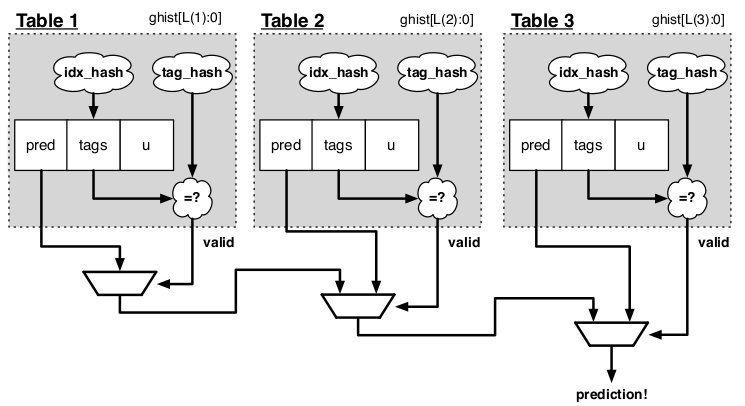
\includegraphics[width=\linewidth]{tage_fig_4_1}
		\bicaption{TAGE预测器。请求地址和全局历史会被输入各个表的索引哈希和标签位哈希函数。然后每个表都会提供它们的预测结果,最后选择拥有最长历史的表。表存储的历史按几何级数逐表递增。\citep{Celio:EECS-2018-151}图4.1.}{The TAGE predictor. The requesting address and the global history are fed into each table’s index hash and tag hash functions. Each table provides its own prediction (or no prediction) and the table with the longest history wins. Each table has geometrically more history bits than the previous table. Figure 4.1 of \citep{Celio:EECS-2018-151}.}
		\label{fig:TAGE}
	\end{figure}
	\item 在目前BIAN的设计中,后端各队列项数的设置都是凭着设计直觉的。正考虑修改各个队列的参数,通过仿真结果来找到各个队列参数最优解。而且出于之前针对rename级提出的两个解决方案带来的时序改善,会考虑多做几项分支跳转的状态回溯备份,并增加乱序执行的指令条数和物理寄存器堆项数。在不断提升处理器性能的同时,也对乱序处理器的设计空间有更深入的探索。
\end{enumerate}
	
	除了一些具体的工作安排,还有一些遥远的展望:
	\begin{enumerate}[label=(\arabic*)]
		\item 通过完善的系统仿真验证,并移植成功Rocket外设和浮点运算部件。最后,能够在FPGA上运行一整套软件栈(如Linux操作系统和GCC编译器),并能够进行SPEC2000/2006的性能测试,在性能上不输RISC-V的BOOM和ARM的Cortex A53,A57系列。
		\item 实现双核的并行。
		\item 目前国内自主研发主流的ISA还是MIPS,肯定会将目前的基于RISC-V的双发射乱序处理器原型机修改为基于MIPS的版本。并且希望能够通过不懈的努力,有朝一日能够将自己的设计真正的流片出来,在实际中得到应用。
	\end{enumerate}
	
	